\documentclass[a4paper,10pt]{article}
\usepackage[utf8]{inputenc}
\usepackage{contmech}
\usepackage{siunitx}
\usepackage{a4wide}
\usepackage{booktabs}
\usepackage{pgfplots}
\pgfplotsset{compat=1.8}
\usepgfplotslibrary{external} 

%\tikzset{external/system call= {lualatex
%                               \tikzexternalcheckshellescape 
%                               -halt-on-error 
%                               -interaction=batchmode
%                               -jobname "\image" "\texsource"}}

%\tikzexternalize


\newcommand{\Co}{\mathrm{Co}}
\newcommand{\WC}{\mathrm{WC}}
\newcommand{\yield}{\mathrm{y}}
\newcommand{\hyd}{\mathrm{hyd}}
\newcommand{\elast}{\mathrm{elast}}
\newcommand{\eq}{\mathrm{V}}


\title{Modeling of thermal stresses in WC-Co allows with realistic microstructures}

\author{Mikael \"Ohman \and Sven Johansson \and G\"oran Wahnstr\"om \and Magnus Ekh}


\begin{document}
\maketitle

\begin{abstract}

\textbf{Keywords}
Cemented carbide composites; Thermal residual stress; Homogenization;
\end{abstract}
% Thermal residual stresses (TRS) were studied in a series of tungsten carbide (WC)–cobalt (Co) composites using neutron powder diffraction. Samples with 10, 20, and 40 wt.\% Co and WC particle sizes of 0.5, 1, 3, and 5 μm were used.
% As expected, the mean WC TRS increased in magnitude as the Co content increased, i.e. as the WC content decreased.
% The corresponding stresses in the Co phase were computed from force balance equilibrium requirements.
% For fixed Co content, the mean (compressive) stresses in the WC increased in magnitude with decreasing WC particle size. The change was most dramatic for the 40 wt.\% Co samples, where the mean TRS increased in magnitude from −440 to −1137 MPa as the WC particle size varied from 5 to 0.5 μm, respectively.
% The stress distribution in the WC phase was studied using the breadths of the WC diffraction peaks.
% The full-width at half-maximum (FWHM) values indicate a broad range of strain within WC particles that increases with increasing stress in the WC and is attributed primarily to point-to-point variation in the angular WC particles.


\section{Introduction}

\section{Theory}
\subsection{Compacted Carbide Builder}

Contiguity...
\begin{figure}[htbp!]
\centering
 \begin{tikzpicture}
 \begin{axis}[
      xmax = 0.35,
      legend pos=north east,
      legend style={draw=none},
      xlabel={Co volume fraction},
      ylabel={Contiguity}
      ]
  \addplot[mark=x, only marks] table[x index=8,y index=3]  {luyckx_table.txt};
  \addlegendentry{Ultra fine}
  \addplot[mark=triangle, only marks] table[x index=8,y index=7]  {luyckx_table.txt};
  \addlegendentry{Fine}
  \addplot[mark=o, only marks] table[x index=8,y index=12]  {luyckx_table.txt};
  \addlegendentry{Medium}
  \addplot[mark=square, only marks] table[x index=8,y index=16]  {luyckx_table.txt};
  \addlegendentry{Coarse}
 \end{axis}
 \end{tikzpicture}
 \caption{Contiguity comparison with experimental data from Luyckx \cite{Lu14}} \label{fig:misorientation_large}
\end{figure}

\end{document}

\subsection{Computational homogenization}

As CCBuilder generates periodic structures, it comes natural to also make use of standard micro-periodic boundary conditions on the generated Representative Volume Element (RVE).
The theory on the micro-periodic boundary condition are detailed in \cite{geers}. 

\section{Results and discussion}

The results are divided into the two parts; the properties of the generated microstructures, followed by the numerical example which uses the generated microstructures to perform an analysis of the thermal residual stresses in a WC-Co system.

\section{Statistical properties}

In order to validate the generated microstructures a few key statistical properties are investigated; grain size distribution, misorientation, and contiguity.

\subsection{Misorientation}
Misorientation is identified at voxel level, and computed for each contacting grain pair.
Trigonal crystallographic symmetries are used when computing the misorientation.

\begin{figure}[htbp!]
\centering
 \begin{tikzpicture}
 \begin{axis}[
      xmin=0, xmax=104.4775,
      legend style={draw=none},
      legend pos=north west,
      xticklabels={0, 0$^{\circ}$ , 20$^{\circ}$, 40$^{\circ}$, 60$^{\circ}$, 80$^{\circ}$, 100$^{\circ}$},
      xlabel={Misorientation},% [${}^{\circ}$]}
      ylabel={Probability density}
      ]
  \addplot[fill=blue!20, draw=none, forget plot, hist={bins=20, density=true, data min=0, data max=104.4775}] table[y index=0]  {misorientation.txt};
  %\addlegendentry{}
  \addplot[densely dashed] table{D3.txt};
  \addlegendentry{Theoretical}
 \end{axis}
 \end{tikzpicture}
 \caption{Generated and theoretical misorientation angle distribution for trigonal symmetry} \label{fig:misorientation_large}
\end{figure}

Figure \ref{fig:misorientation_large} show the distribution or a very large system, containing 13012 grains, in good agreement with the theoretical results from \cite{orientations_2004}.
These results can be used to verify numerically that the random placement of grains are not skewing the misorientation.

%%%%%%%%%%%%%%%%%%%%%%%%%%%%%%%%%%%%%%%%%%%%%%%%%%%%%%%%%%%%%%%%%%%%%%%%%%%%%%%%%%%%%%
\subsection{Grain size distribution}

\begin{figure}[htbp!]
\centering
 \begin{tikzpicture}
 \begin{axis}[
      %xmin=0, xmax=104.4775,
      legend style={draw=none},
      xlabel={Grain volume fraction},% [${}^{\circ}$]}
      ylabel={Probability density}
      ]
  \addplot[fill=blue!20, draw=none, hist={bins=20, density=true}] table[y index=0]  {grain_volumes.txt};
 \end{axis}
 \end{tikzpicture}
 \caption{Distribution of normed generated grain volumes} \label{fig:grain_volumes}
\end{figure}

Figure \ref{fig:grain_volumes} show the distribution of grain volumes (relative the largest grain) very large system, containing 13012 grains and 17.8\% Co by volume.
The distribution can primarily be adjusted by modifying the original grain sizes before overlaps are removed.

%%%%%%%%%%%%%%%%%%%%%%%%%%%%%%%%%%%%%%%%%%%%%%%%%%%%%%%%%%%%%%%%%%%%%%%%%%%%%%%%%%%%%%
\subsection{Contiguity}


%%%%%%%%%%%%%%%%%%%%%%%%%%%%%%%%%%%%%%%%%%%%%%%%%%%%%%%%%%%%%%%%%%%%%%%%%%%%%%%%%%%%%%
\subsection{Residual stresses}

 % Data generated from paraviews CSV-files
% d = np.loadtxt('wc_phase.csv', skiprows=1, delimiter=',');       np.savetxt('wc_vol.txt',       d[::8,-2]); np.savetxt('wc_hyd.txt',       np.sum(d[::8,[0,5,8]], 1)/3 * 1e-9); np.savetxt('wc_vm.txt',       d[::8,18] * 1e-9); print(np.mean(d[:,[0,5,8]]) * 1e-9)
% d = np.loadtxt('wc_phase_elast.csv', skiprows=1, delimiter=','); np.savetxt('wc_vol_elast.txt', d[::8,-2]); np.savetxt('wc_hyd_elast.txt', np.sum(d[::8,[0,5,8]], 1)/3 * 1e-9); np.savetxt('wc_wm_elast.txt', d[::8,18] * 1e-9); print(np.mean(d[:,[0,5,8]]) * 1e-9)
% d = np.loadtxt('co_phase.csv', skiprows=1, delimiter=',');       np.savetxt('co_vol.txt',       d[::2,-2]); np.savetxt('co_hyd.txt',       np.sum(d[::2,[0,5,8]], 1)/3 * 1e-9); np.savetxt('co_wm.txt',       d[::2,18] * 1e-9); print(np.mean(d[:,[0,5,8]]) * 1e-9)
% d = np.loadtxt('co_phase_elast.csv', skiprows=1, delimiter=','); np.savetxt('co_vol_elast.txt', d[::2,-2]); np.savetxt('co_hyd_elast.txt', np.sum(d[::2,[0,5,8]], 1)/3 * 1e-9); np.savetxt('co_wm_elast.txt', d[::2,18] * 1e-9); print(np.mean(d[:,[0,5,8]]) * 1e-9)

For the cobalt phase, the thermal and elastic properties are set to \cite{rohrer_2007???}
\begin{align*}
\alpha &= \SI{13.8e-6}{\per\kelvin}
\\
\nu &= \num{0.31}
\\
E &= \SI{211}{\giga\pascal}.
\end{align*}
The plastic material parameters will be highly dependent on temperature and carbon infusion, it is difficult to ascertain accurate plastic parameters.
In the simulations with elastoplastic models for cobalt the yield stress and hardening are set to $\sigma_\yield = \SI{350}{\mega\pascal}$, $H = \SI{20}{\giga\pascal}$ \cite{}.


The WC-phase are modeled with anisotropic elasticity taken from \cite{rohrer_2007}, 
\begin{align*}
  C_{11} = \SI{720}{\giga\pascal}\\
  C_{12} = \SI{254}{\giga\pascal}\\
  C_{13} = \SI{267}{\giga\pascal}\\
  C_{33} = \SI{972}{\giga\pascal}\\
  C_{44} = \SI{328}{\giga\pascal}
\end{align*}
with thermal expansion coefficients
\begin{align*}
\alpha_1 = \alpha_2 &= \SI{5.2e-6}{\per\kelvin} \\
\alpha_3 &= \SI{7.3e-6}{\per\kelvin}
\end{align*}
where the anisotropy is oriented according to each WC-grain.


\begin{figure}[htbp!]
\centering
 %\includegraphics[width=0.5\linewidth]{RVE_grains}
 \caption{Microstructure used in finite element analysis} \label{fig:rve_grains}
\end{figure}

\begin{figure}[htbp!]
\centering
\begin{tikzpicture}
 \begin{axis}[
      width=0.45\linewidth,
      xmin=-2.5, xmax=2.5,
      legend style={draw=none},
      legend pos=north west,
      xlabel={Hydrostatic stress ($\sigma_{\hyd}$) [GPa]},
      ylabel={Probability density}
      ]
  \addplot[fill=blue, draw=blue, very thick, opacity=0.3, draw=none, hist={bins=80, density=true}] table[y index=0]  {co_hyd.txt};
  \addlegendentry{Co}
  \addplot[fill=red, draw=red, very thick, opacity=0.3, draw=none, hist={bins=80, density=true}] table[y index=0]  {wc_hyd.txt};
  \addlegendentry{WC}
 \end{axis}
 \end{tikzpicture}
 \begin{tikzpicture}
 \begin{axis}[
      width=0.45\linewidth,
      xmin=0, xmax=3.5,
      ymax=1.5,
      legend style={draw=none},
      legend pos=north east,
      xlabel={Hydrostatic stress ($\sigma_{\eq}$) [GPa]},
      ylabel={Probability density}
      ]
  \addplot[fill=blue, draw=blue, very thick, opacity=0.3, draw=none, hist={bins=320, density=true}] table[y index=0]  {co_vm.txt};
  \addlegendentry{Co}
  \addplot[fill=red, draw=red, very thick, opacity=0.3, draw=none, hist={bins=80, density=true}] table[y index=0]  {wc_vm.txt};
  \addlegendentry{WC}
 \end{axis}
 \end{tikzpicture}

  %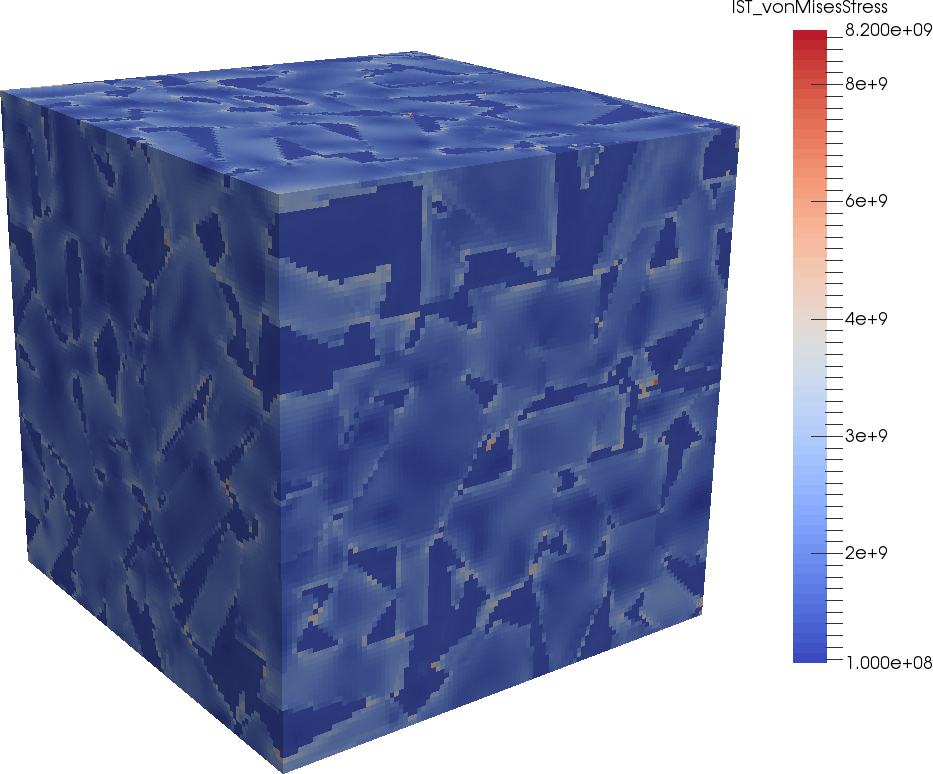
\includegraphics[width=0.4\linewidth]{rve_vonmises}
 \caption{Hydrostatic and von Mises equivalent stresses using a elasto-plastic Co-model} \label{fig:rve_stress}
\end{figure}

\begin{figure}[htbp!]
\centering
 \begin{tikzpicture}
 \begin{axis}[
      width=0.45\linewidth,
      xmin=-2.5, xmax=2.5,
      legend style={draw=none},
      legend pos=north west,
      xlabel={Hydrostatic stress ($\sigma_{\hyd}$) [GPa]},
      ylabel={Probability density}
      ]
  \addplot[fill=blue, draw=blue, very thick, opacity=0.3, draw=none, hist={bins=80, density=true}] table[y index=0]  {co_hyd_elast.txt};
  \addlegendentry{Co}
  \addplot[fill=red, draw=red, very thick, opacity=0.3, draw=none, hist={bins=80, density=true}] table[y index=0]  {wc_hyd_elast.txt};
  \addlegendentry{WC}
 \end{axis}
 \end{tikzpicture}
 \begin{tikzpicture}
 \begin{axis}[
      width=0.45\linewidth,
      xmin=0, xmax=3.5,
      ymax=1.5,
      legend style={draw=none},
      legend pos=north east,
      xlabel={Hydrostatic stress ($\sigma_{\hyd}$) [GPa]},
      ylabel={Probability density}
      ]
  \addplot[fill=blue, draw=blue, very thick, opacity=0.3, draw=none, hist={bins=80, density=true}] table[y index=0]  {co_vm_elast.txt};
  \addlegendentry{Co}
  \addplot[fill=red, draw=red, very thick, opacity=0.3, draw=none, hist={bins=80, density=true}] table[y index=0]  {wc_vm_elast.txt};
  \addlegendentry{WC}
 \end{axis}
 \end{tikzpicture}
 %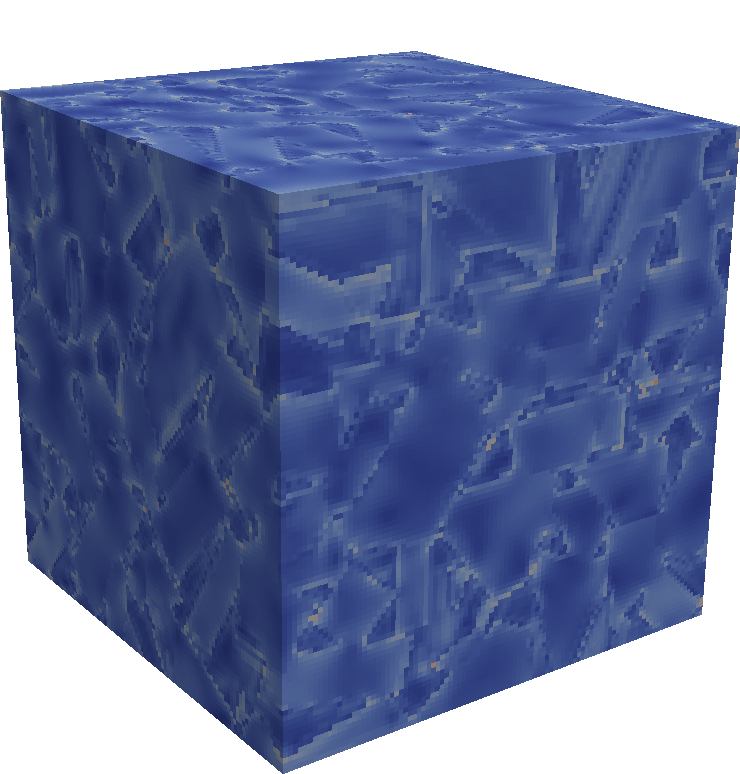
\includegraphics[width=0.4\linewidth]{rve_vonmises_elastic}
 \caption{Hydrostatic and von Mises equivalent stresses using a elastic Co-model} \label{fig:rve_stress_elastic}
\end{figure}


\begin{figure}[htbp!]
\centering
  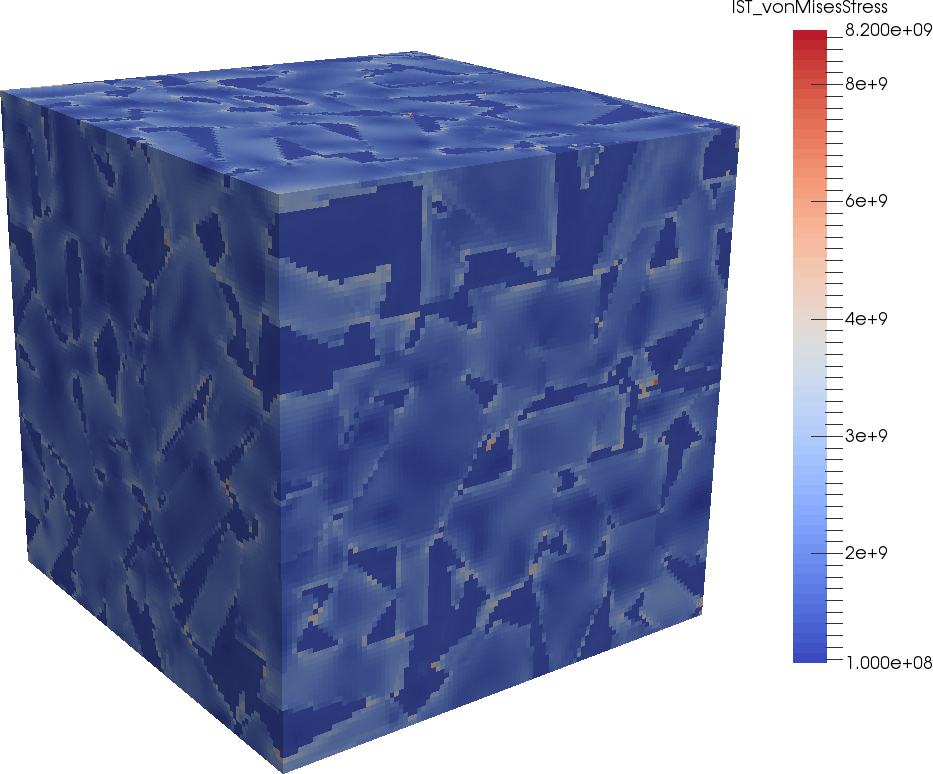
\includegraphics[scale=0.25]{rve_vonmises}
  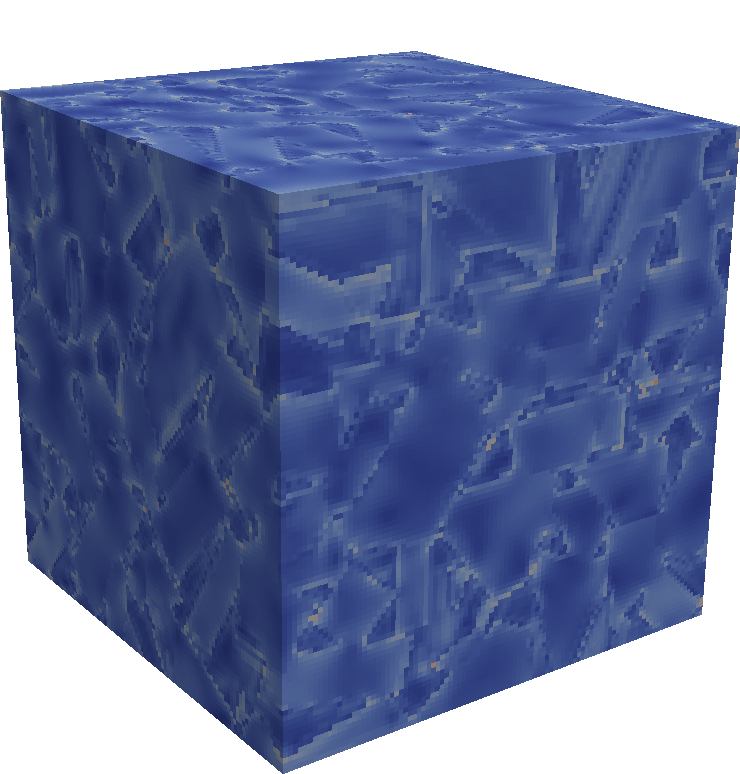
\includegraphics[scale=0.25]{rve_vonmises_elastic}
 \caption{Comparison of stress distribution with elasto-plastic (left) and elastic (right) cobalt phase} \label{fig:rve_stress}
\end{figure}

% \begin{figure}[htbp!]
% \centering
%  \caption{Distribution of volumetric strain using a elasto-plastic Co-model} \label{fig:rve_vol_dist}
% \end{figure}
% 
% \begin{figure}[htbp!]
% \centering
%  \begin{tikzpicture}
%  \begin{axis}[
%       xmin=-0.035, xmax=-0.01,
%       legend style={draw=none},
%       legend pos=north west,
%       xlabel={Volumetric strain ($\epsilon_{\vol}$)},
%       ylabel={Probability density}
%       ]
%   \addplot[fill=blue, draw=blue, very thick, opacity=0.3, draw=none, hist={bins=80, density=true}] table[y index=0]  {co_vol.txt};
%   \addlegendentry{Co (plastic)}
%   \addplot[fill=red, draw=red, very thick, opacity=0.3, draw=none, hist={bins=80, density=true}] table[y index=0]  {wc_vol.txt};
%   \addlegendentry{WC (plastic)}
%  \end{axis}
%  \end{tikzpicture}
%  
%  \begin{tikzpicture}
%  \begin{axis}[
%       xmin=-0.035, xmax=-0.01,
%       legend style={draw=none},
%       legend pos=north west,
%       xlabel={Volumetric strain ($\epsilon_{\vol}$)},
%       ylabel={Probability density}
%       ]
%   \addplot[fill=blue, draw=blue, very thick, opacity=0.3, draw=none, hist={bins=80, density=true}] table[y index=0]  {co_vol_elast.txt};
%   \addlegendentry{Co (elastic)}
%   \addplot[fill=red, draw=red, very thick, opacity=0.3, draw=none, hist={bins=80, density=true}] table[y index=0]  {wc_vol_elast.txt};
%   \addlegendentry{WC (elastic)}
%  \end{axis}
%  \end{tikzpicture}
%  \caption{Distribution of total volumetric strain using a elastic Co-model} \label{fig:rve_vol_dist_elastic}
% \end{figure}


To compare with experimental results from Mari et.\ al \cite{mari09} the numerical examples are set up with \SI{17.7}{\percent} cobalt (by volume).
The Representative Volume Element (RVE) shown in figure \ref{fig:rve_grains} contains 164 WC-grains discretized in a $100^3$ grid and is subject to standard micro-periodic boundary conditions, cf.\ Geers et al.\ \cite{geers}.
Denser grids quickly leads to excessively expensive analysis, which means there is a trade-off of number of grains and sufficient resolution.
The analysis solves for zero macroscopic stress as to simulate the cooling process in free sintering.
Experimental results from \cite{mari09} show onset of residual stresses at +\SI{800}{\kelvin}, and the temperature difference $\Delta T = \SI{800}{\kelvin}$ is used for the stress free state in all simulations.


\begin{table}
\centering
\caption{Comparison of hydrostatic and effective stress [\si{\mega\pascal}]}\label{tab:stress_comparison}
\begin{tabular}{l|r|r||r|r}
                           & Plastic Co & Elastic Co & Mari et al. \cite{mari09} & Exnar et al. \cite{exnar92}\\
                           \midrule
 $\bar{\sigma}_{\WC,\hyd}$ & $ -222 \pm 513 $          & $ -262 \pm 473 $ & $ -400 $ & $ -210\pm110 $\\
 $\bar{\sigma}_{\Co,\hyd}$ & $ 1030 \pm 816 $          & $ 1216 \pm 948 $ & $ 1847 $ & $ 1330\pm150 $\\
 $\bar{\sigma}_{\WC,\eq}$  & $ 1301 \pm 595 $          & $ 1234 \pm 573 $ &          & $  700\pm320 $\\
 $\bar{\sigma}_{\Co,\eq}$  & $ 430 \pm \phantom{0}54 $ & $ 1043 \pm 385 $ &          & $  950\pm480 $\\
\end{tabular}
\end{table}

% WC only Hyd: -5.02421747974e-05 \pm 171.810779382                                                                                                                                     
% WC only eq: 444.593432029 \pm 191.563218737


Comparisons of the stress distribution with from Mari et al.\ (2009) \cite{mari09} and Exnar et al.\ (1992) \cite{exnar92}, and Coats et al.\ (2003) \cite{Coats_2003} are summarized in table \ref{tab:stress_comparison}.
Exnar et al.\ performed a 2D elastic finite element analysis on a small unit cell containing around 17 grains. Mari et al.\ measured the temperature dependence by neutron diffraction, where values for a temperature difference of $800\si{\degree}$ has been extracted.



% With the plastic behavior for the cobalt phase, the average hydrostatic stresses are $\bar{\sigma}_{\WC,\hyd} = -0.22 \si{\giga\pascal}$ and $\bar{\sigma}_{\Co,\hyd} = 1.00 \si{\giga\pascal}$, matched by the peaks in the distributions shown in  figure \ref{fig:rve_stress}.
% In the elastic case, figure \ref{fig:rve_stress_elastic}, the average hydrostatic stresses are $\bar{\sigma}_{\WC,\hyd,\elast} = -0.26 \si{\giga\pascal}$ and $\bar{\sigma}_{\Co,\hyd,\elast} = 1.20 \si{\giga\pascal}$.

Comparing the effective (von Mises) stresses in figure \ref{fig:rve_stress} and \ref{fig:rve_stress_elastic} one can see that the plastic versus elastic model for cobalt has a small effect on the WC phase.


\section{Conclusions}

Future work to mention:
\begin{itemize}
 \item \cite{Coats_2003} grain size dependence; Not captured in current model. Could possibly be captured by interface modeling.
 \item No temperature dependence; Solidification of Co is assumed to happen 800\si{\degree}.
\end{itemize}

In the analysis, the major limitation is the lack of temperature dependent material data, however, the plastic response in the cobalt phase does not have a significant effect on the stress state in the WC grains.


\end{document}
